\subsection{Convolution engine}
In this section we will describe the convolution engine which is at the heart of the FPGA architecture.
We will first describe the convolution engine as a stream processor seen from the outside system, before showing how the convolution engine works on a conceptual basis.
Lastly we will show how the convolution engine is implemented.

\subsection{The convolution engine as a component}
A design goal for our system was to reconfigure the FPGA depending on the task, which necessitates synthesizing several versions of our architecture so that the correct architecture may be chosen at run time.
In addition to using several architectures, each version is also programmable, allowing the kernel values, map operators and reduce operators to be programmed at runtime.
In order to achive this we parametrized our design, allowing us to generate different architectures by simply changing a parameter once.
The parameters available are:

\begin{description}
    \item[Kernel dimensions] \hfill \\
        The most fundamental parameter in our design, the kernel dimension dictates how many pixels we need to calculate a single output pixel.
        This is very fundamental parameter, and we will see how setting the kernel dimension will effect other important sizes in our system as we explore the system.
    \item[Image input width] \hfill \\
        The width which input image data is presented 
    \item[Pixel width] \hfill \\
        The width of each pixel. When image input width and pixel width does not match, for instance with 16 bit input width and 24 bit pixel width, the convolution engine must buffer and translate the input stream 
    \item[Control input width] \hfill \\
        As with input data width, the convolution engine must know the width of the incoming control data.
    \item[Image output width] \hfill \\
        The data width that the convolution engine should output. As with input, translating widths is nescessary.
\end{description}

By parametrizing the convolution engine we can view it as any other processor module with the following inputs and outputs:

% \begin{tabular}{ l | l | l }
% \multicolumn{2}{c}{Input}
%     \hline
%     Signal & Width\\
%     \hline
%     Image data in           & Image input width     & Data stream from camera on row format \\
%     Image data valid        & 1                     & image data input is valid\\
%     Control data in         & Control data width    & Data stream from MCU\\
%     Control data valid      & 1                     & MCU data is valid\\
%     Request image data      & 1                     & Current output data is recieved\\
%     Reset                   & 1                     & Convolution engine should reset
% \end{tabular}
% 
% \begin{tabular}{ l | l | l}
%     \multicolumn{2}{c}{Output}
%     \hline
%     Signal & Width\\
%     \hline
%     Image data out          & Image input width     & The processed image data on row format\\
%     Image data valid        & 1                     & Current output data is valid
% \end{tabular}

To the outside system the convolution engine is now a module that once programmed operates on a data stream of an image and outputting a processed stream. 
By using valid signals the outside system can provide data at any pace, and throttle the output by requesting data when the convolution engine indicates that data is ready. 

\subsection{A conceptual overview}
In this section we provide a conceptual description of how convolution is performed in our system.

\subsubsection{Data input}
We will first discuss how image data is presented to the processor at the core of the convolution engine.
Fig \ref{daisy_processing.pdf}1 shows how the convolution engine buffers rows from the image input until it has accumulated enough rows.
These rows form a \textit{Sweep}, which is fed into the processor as a series of column slices.
We have now established how the processor is fed data from the convolution engine, and we can now explore what happens inside the processor.

\begin{figure}[h!]
    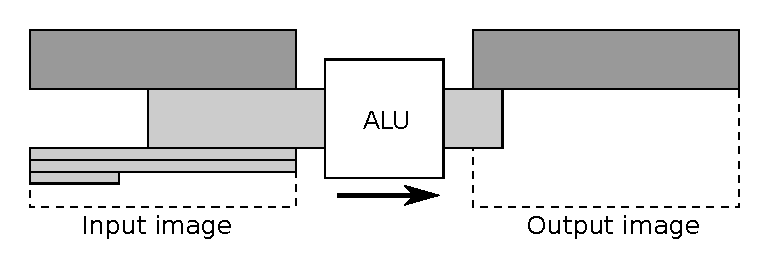
\includegraphics[width=\linewidth]{img/daisy_processing.pdf}
    \caption{TODO}
    \label{fig:sweep_feed}
\end{figure}

\subsubsection{The sweep frontier}
As shown in \ref{fig:sweep_feed}, each sweep is fed through the processor as a data stream.
This stream of pixel data is again buffered in a special register file called the \textit{conveyor belt}.
The purpose of the conveyor belt is to maintain the \textit{sweep frontier}, consisting of the most recent data from the current sweep.
The conveyor has several rows of registers, representing the \textit{sweep depth}, each row as wide as a column slice, representing the \textit{sweep width}.
Figures \ref{frontier1} and \ref{frontier2} show the sweep window for a 3x3 convolution.
Recall from the background section how the dimensions of the kernel dictates the size of each pixels neighbourhood.
In \ref{frontier1} we see that the seven middle pixels, marked as gray, have access to their entire neighbourhood.
By letting the frontier depth equal the kernel dimension, the middle row will always have access to their whole neighbourhood, explaining the purpose of the sweep depth.
Had we used a 5x5 kernel instead we would have had a sweep depth of 5, again making it possible to have the entire neighbourhood in memory.
Had we used a a kernel with size 5x5 we would need a depth of 5 to simultaneously keep each neighbour in the conveyor, which is why kernel size acts as a paramater before synthesizing, allowing the design to be tailored to one kernel size.
We now see the benefit of having a sweep depth similar to the kernel dimension, but what about the sweep width, how wide should it be, and why?
To answer this we must take a deeper look at the conveyor and ALU.
\clearpage
\begin{figure}[h!]
    \centering
    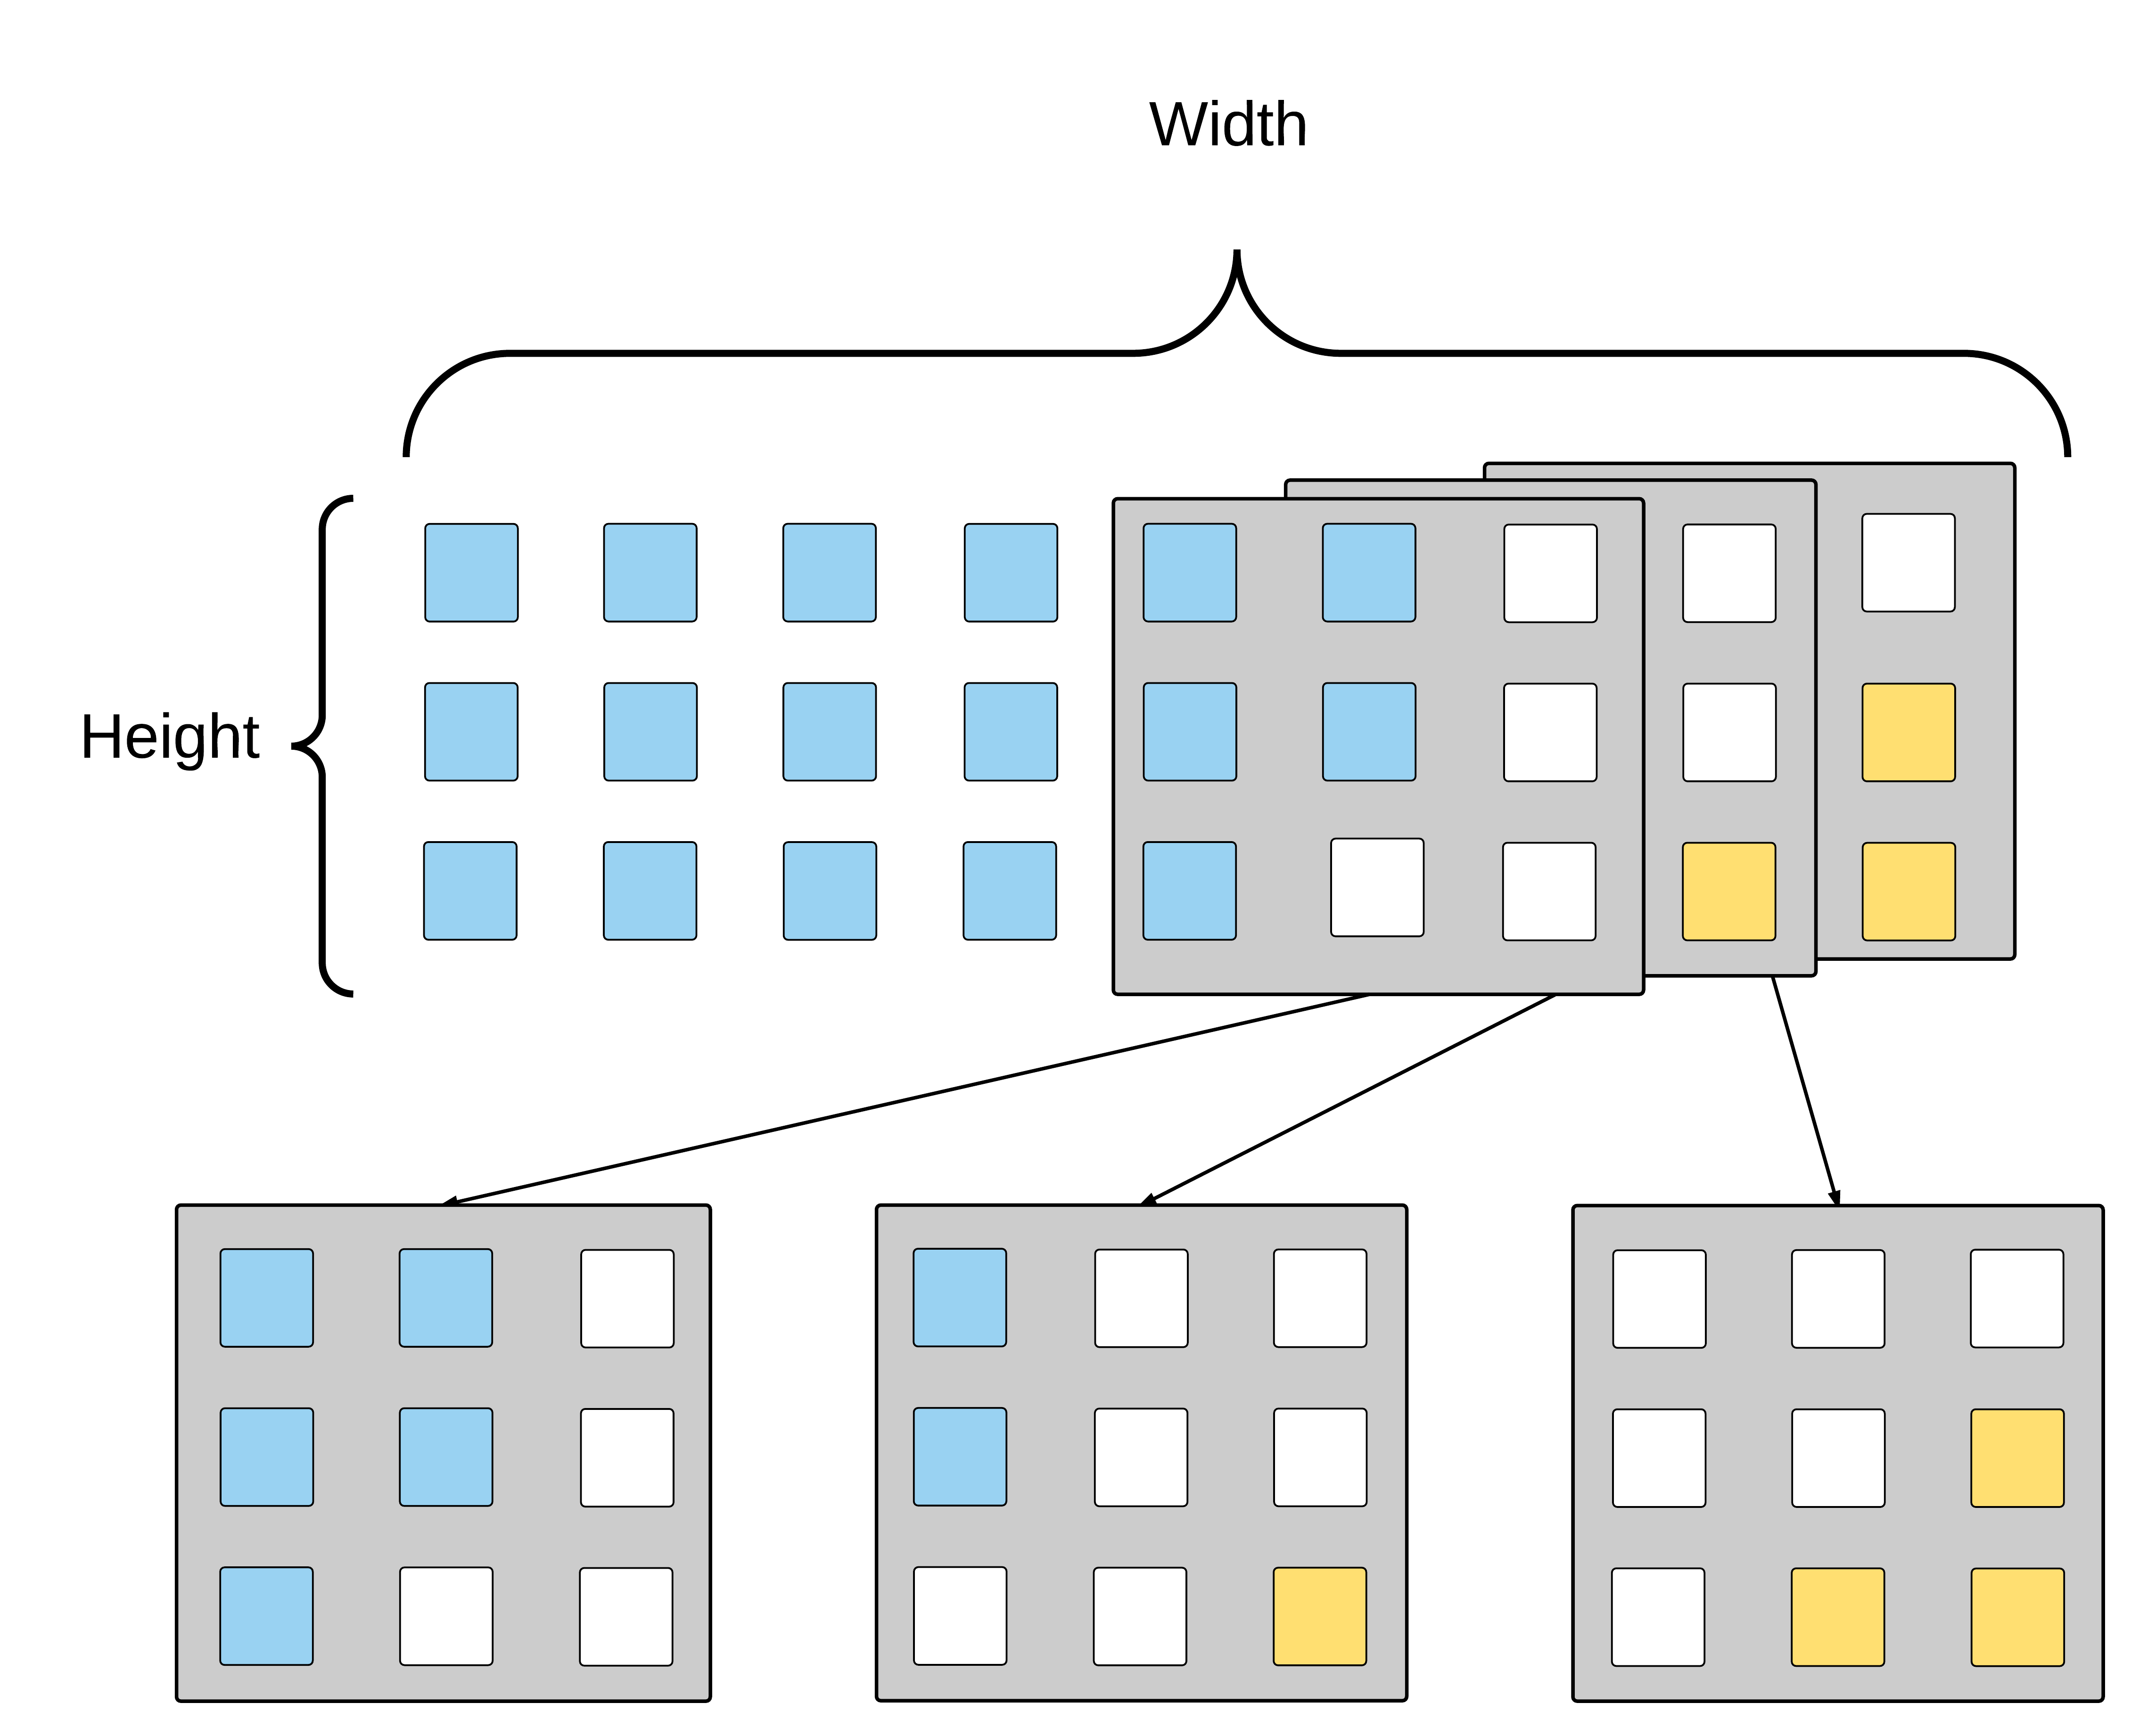
\includegraphics[width=10cm]{img/frontier1.png}
    \caption{The frontier. The three rightmost pixels are shown with its full neighbourhood, which overlaps with its neighbours.}
    \label{fig:frontier1}
\end{figure}

\begin{figure}[h!]
    \centering
    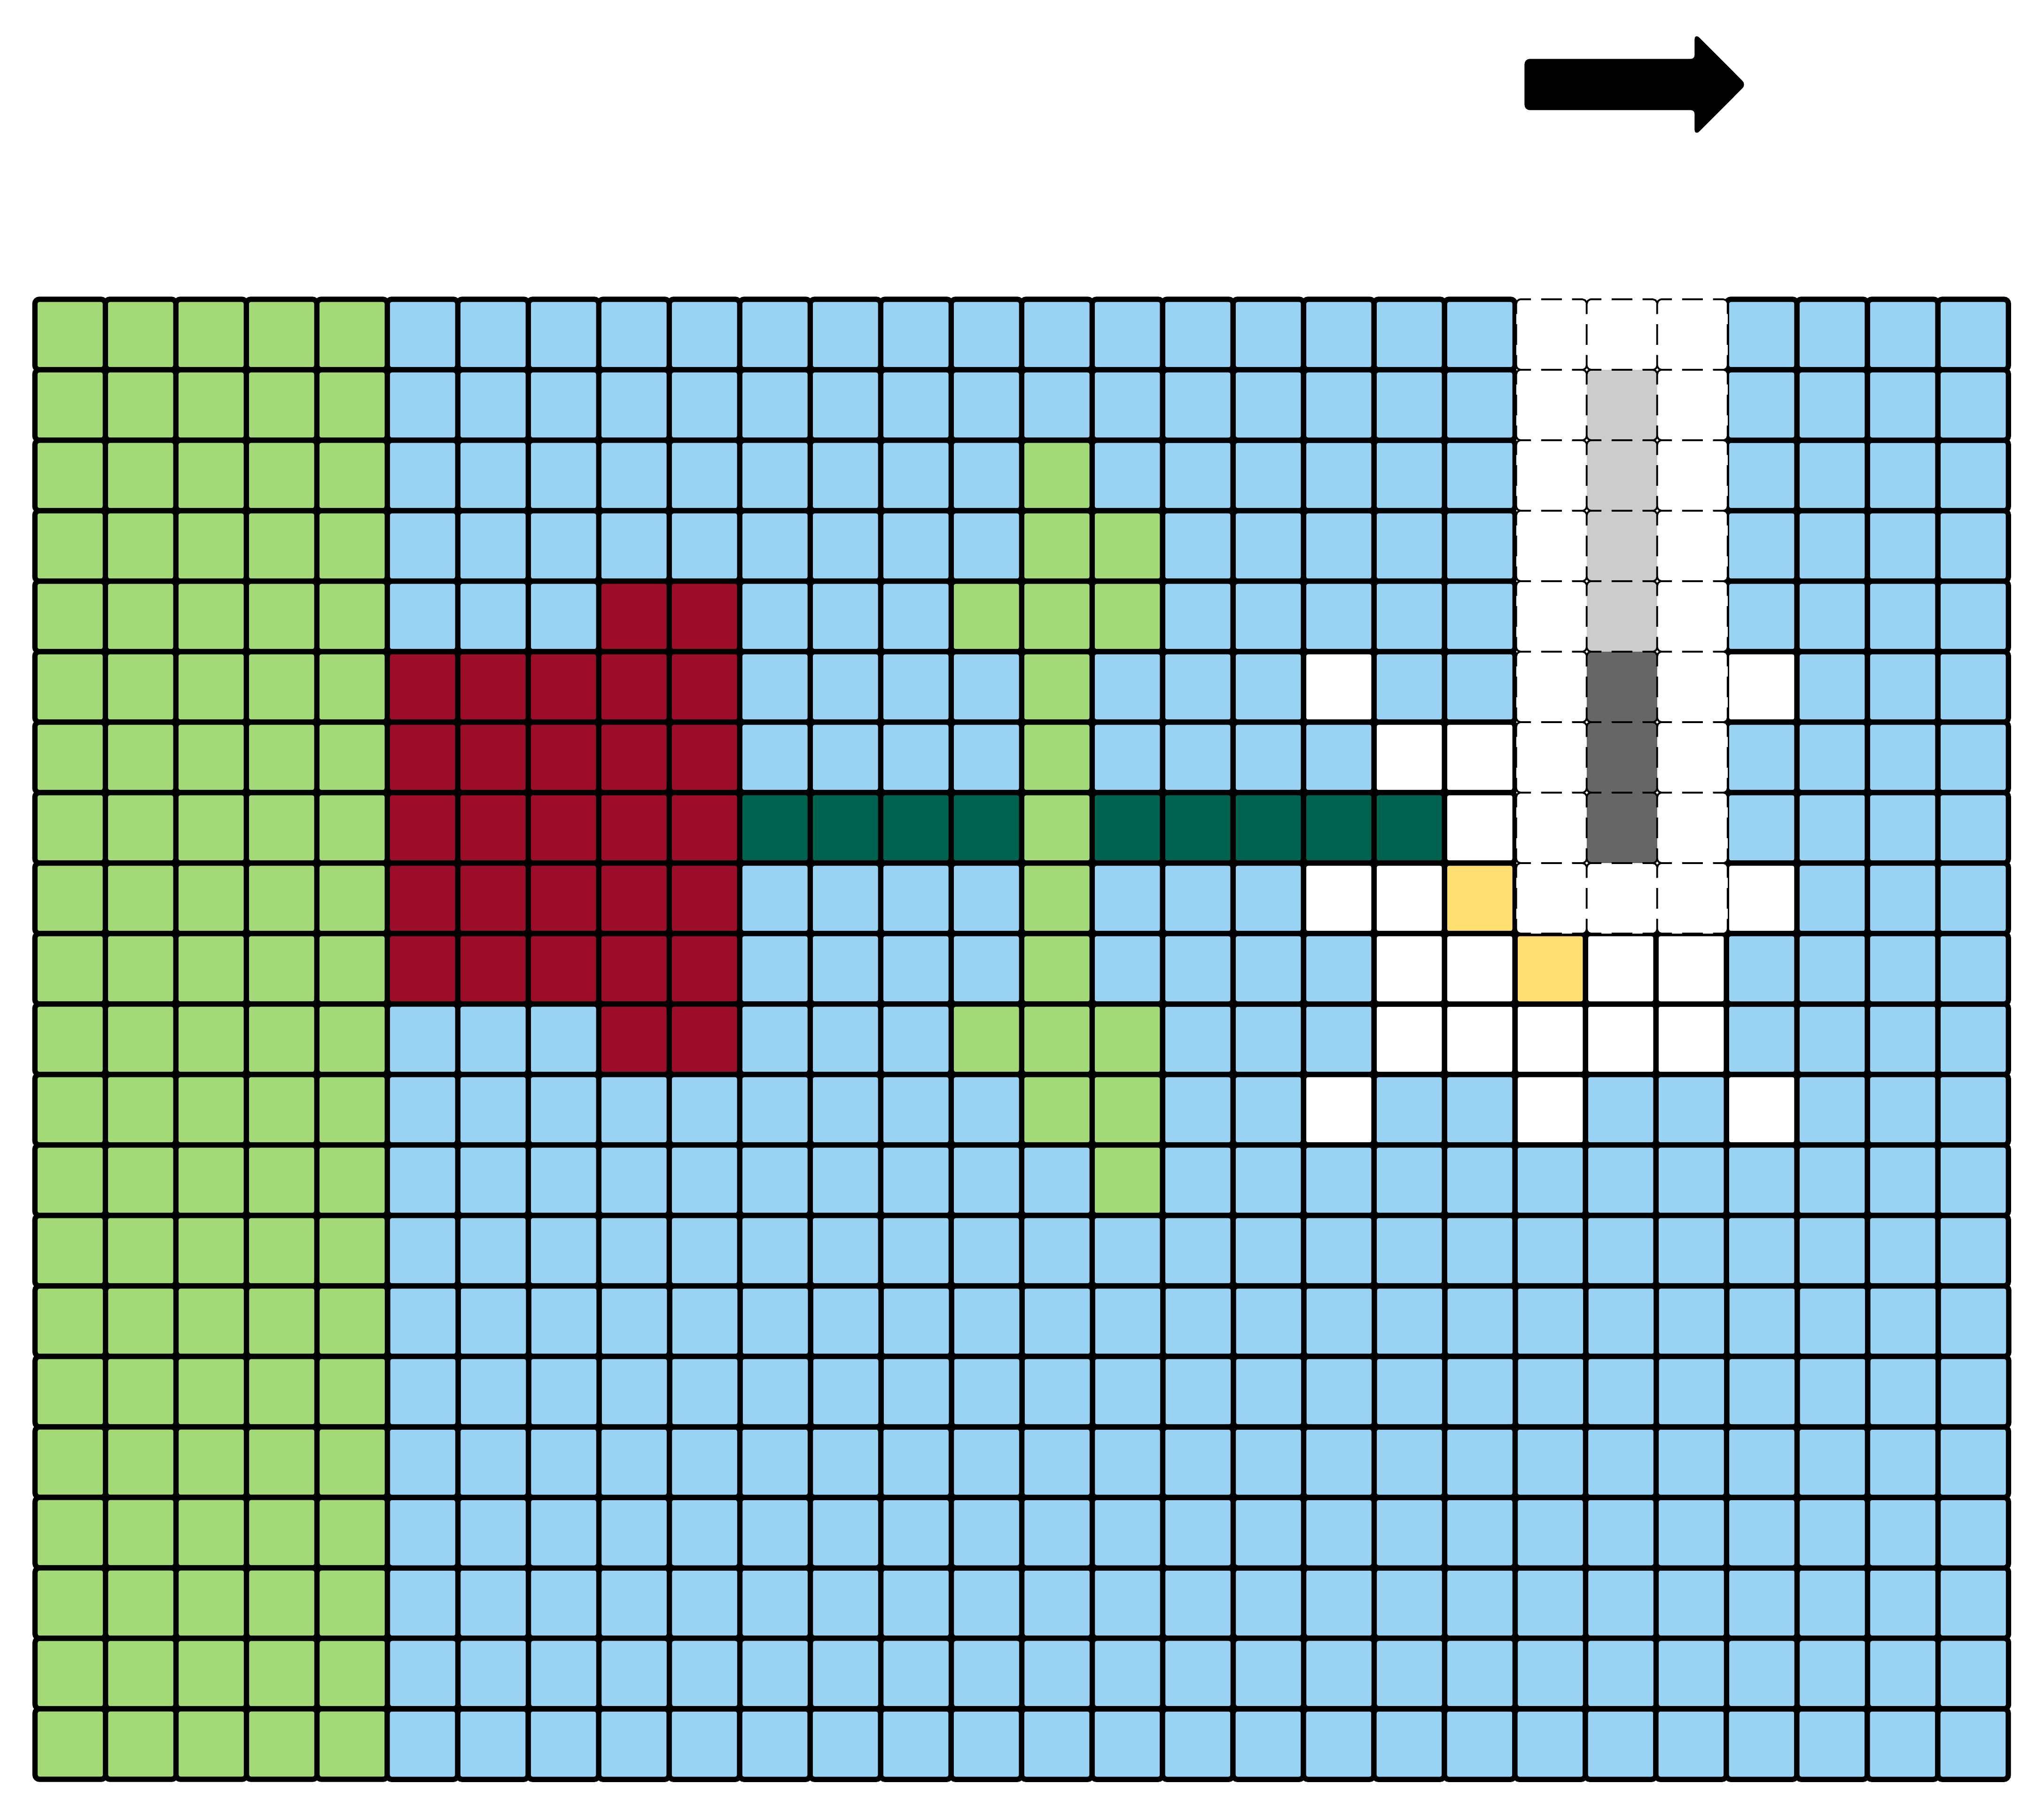
\includegraphics[width=10cm]{img/frontier2.png}
    \caption{The image from which the frontier in the previous figure is taken.}
    \label{fig:frontier2}
\end{figure}

\subsubsection{Processing pixels}
Again, recall from the background section that each output pixel is the result of each neighbour pixel being mapped with its associated kernel and reduced with accumulated value.
With a 3x3 kernel this means we need at least nine cycles per pixel, and with 5x5 we would need 25.
Ideally we want to output a pixel each cycle, which is why we use a row of ALUs, each consisting of a mapping unit and a reduction unit, allowing us to process several pixels simultaneously.
Fig \ref{frontier1} shows how the leftmost and rightmost pixels lack the nescessary neighbours, so it makes sense to have as many ALUs as the sweep width, minus the mantle.
For a 5x5 convolution, the mantle would be of size 2, meaning that.

To explain how pixels are processed we will consider a 3x3 kernel.
Each pixel that enters the conveyor is part of 9 neighbourhoods, and should be used in 9 mapping operations.
Ideally the processor should accept one pixel each clock cycle, and conversively it should have a processed pixel ready each cycle, apart from the border pixels which does not have sufficent neighbours.


A natural frontier width, and the one we use, would be as wide as the square of the kernel dimension, 9 in the case of a 3x3 kernel.
To see why this number is special we see what happens if the processor runs optimally.
In this case, running optimally means each pixel is used nine times, and that a new pixel may be accepted every cycle.
By accepting a new pixel in the conveyor every cycle we can now only keep a pixel in its current row for nine cycles, and as long as each pixel is used every cycle a processed pixel should be ready.

\subsection{Overview}
The overall design of our convolution processor, named "Daisy", shown in Figure \ref{fig:Convolution} consists of four main modules with the following responsibilities as follows:
\begin{figure}[h!]
    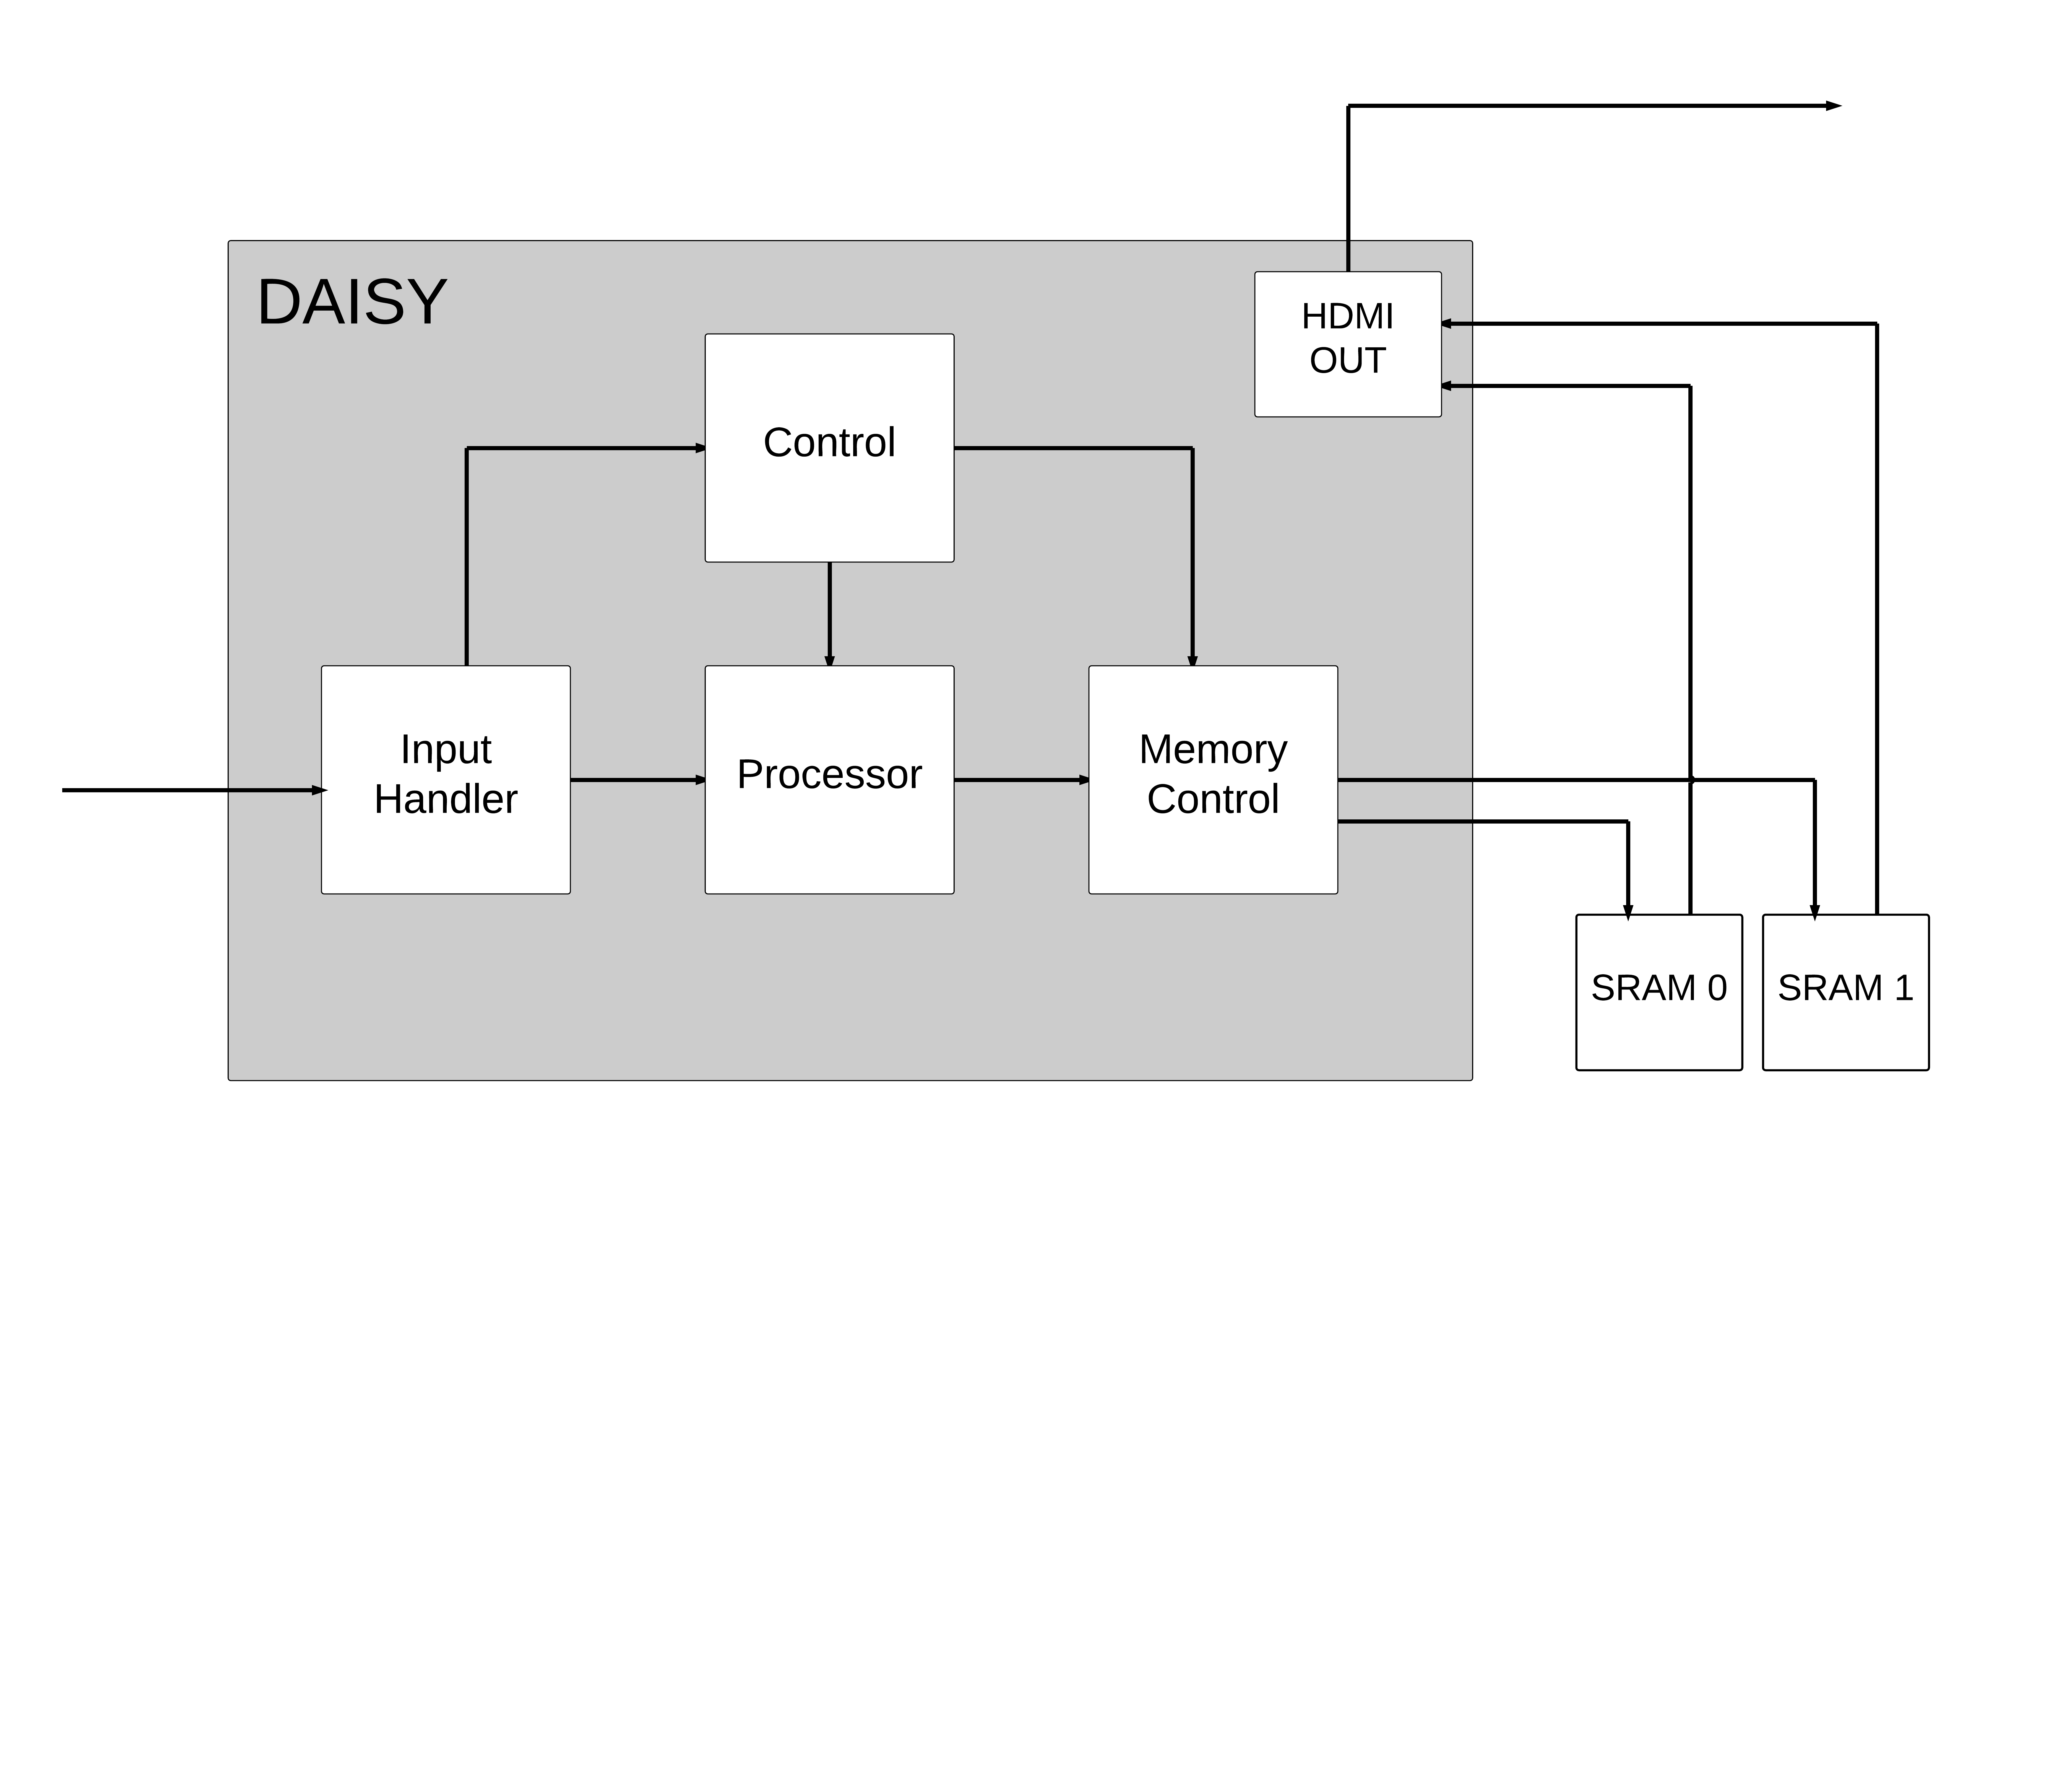
\includegraphics[width=\linewidth]{img/daisy_overview.png}
    \caption{The data path for our processor, named Daisy after the way it daisy chains many control signals.}
    \label{fig:Convolution}
\end{figure}

\begin{description}
    \item[Input Handler] \hfill\\ 
        The interface between the data stream and our processor is responsible for gathering data from a wide variety of input streams of different bandwidths and speeds and present this data to the processor as a continuous data stream with a fixed width.
        In order to do this the input handler must be able to translate from any input width to the desired output width.

\begin{figure}[h!]
    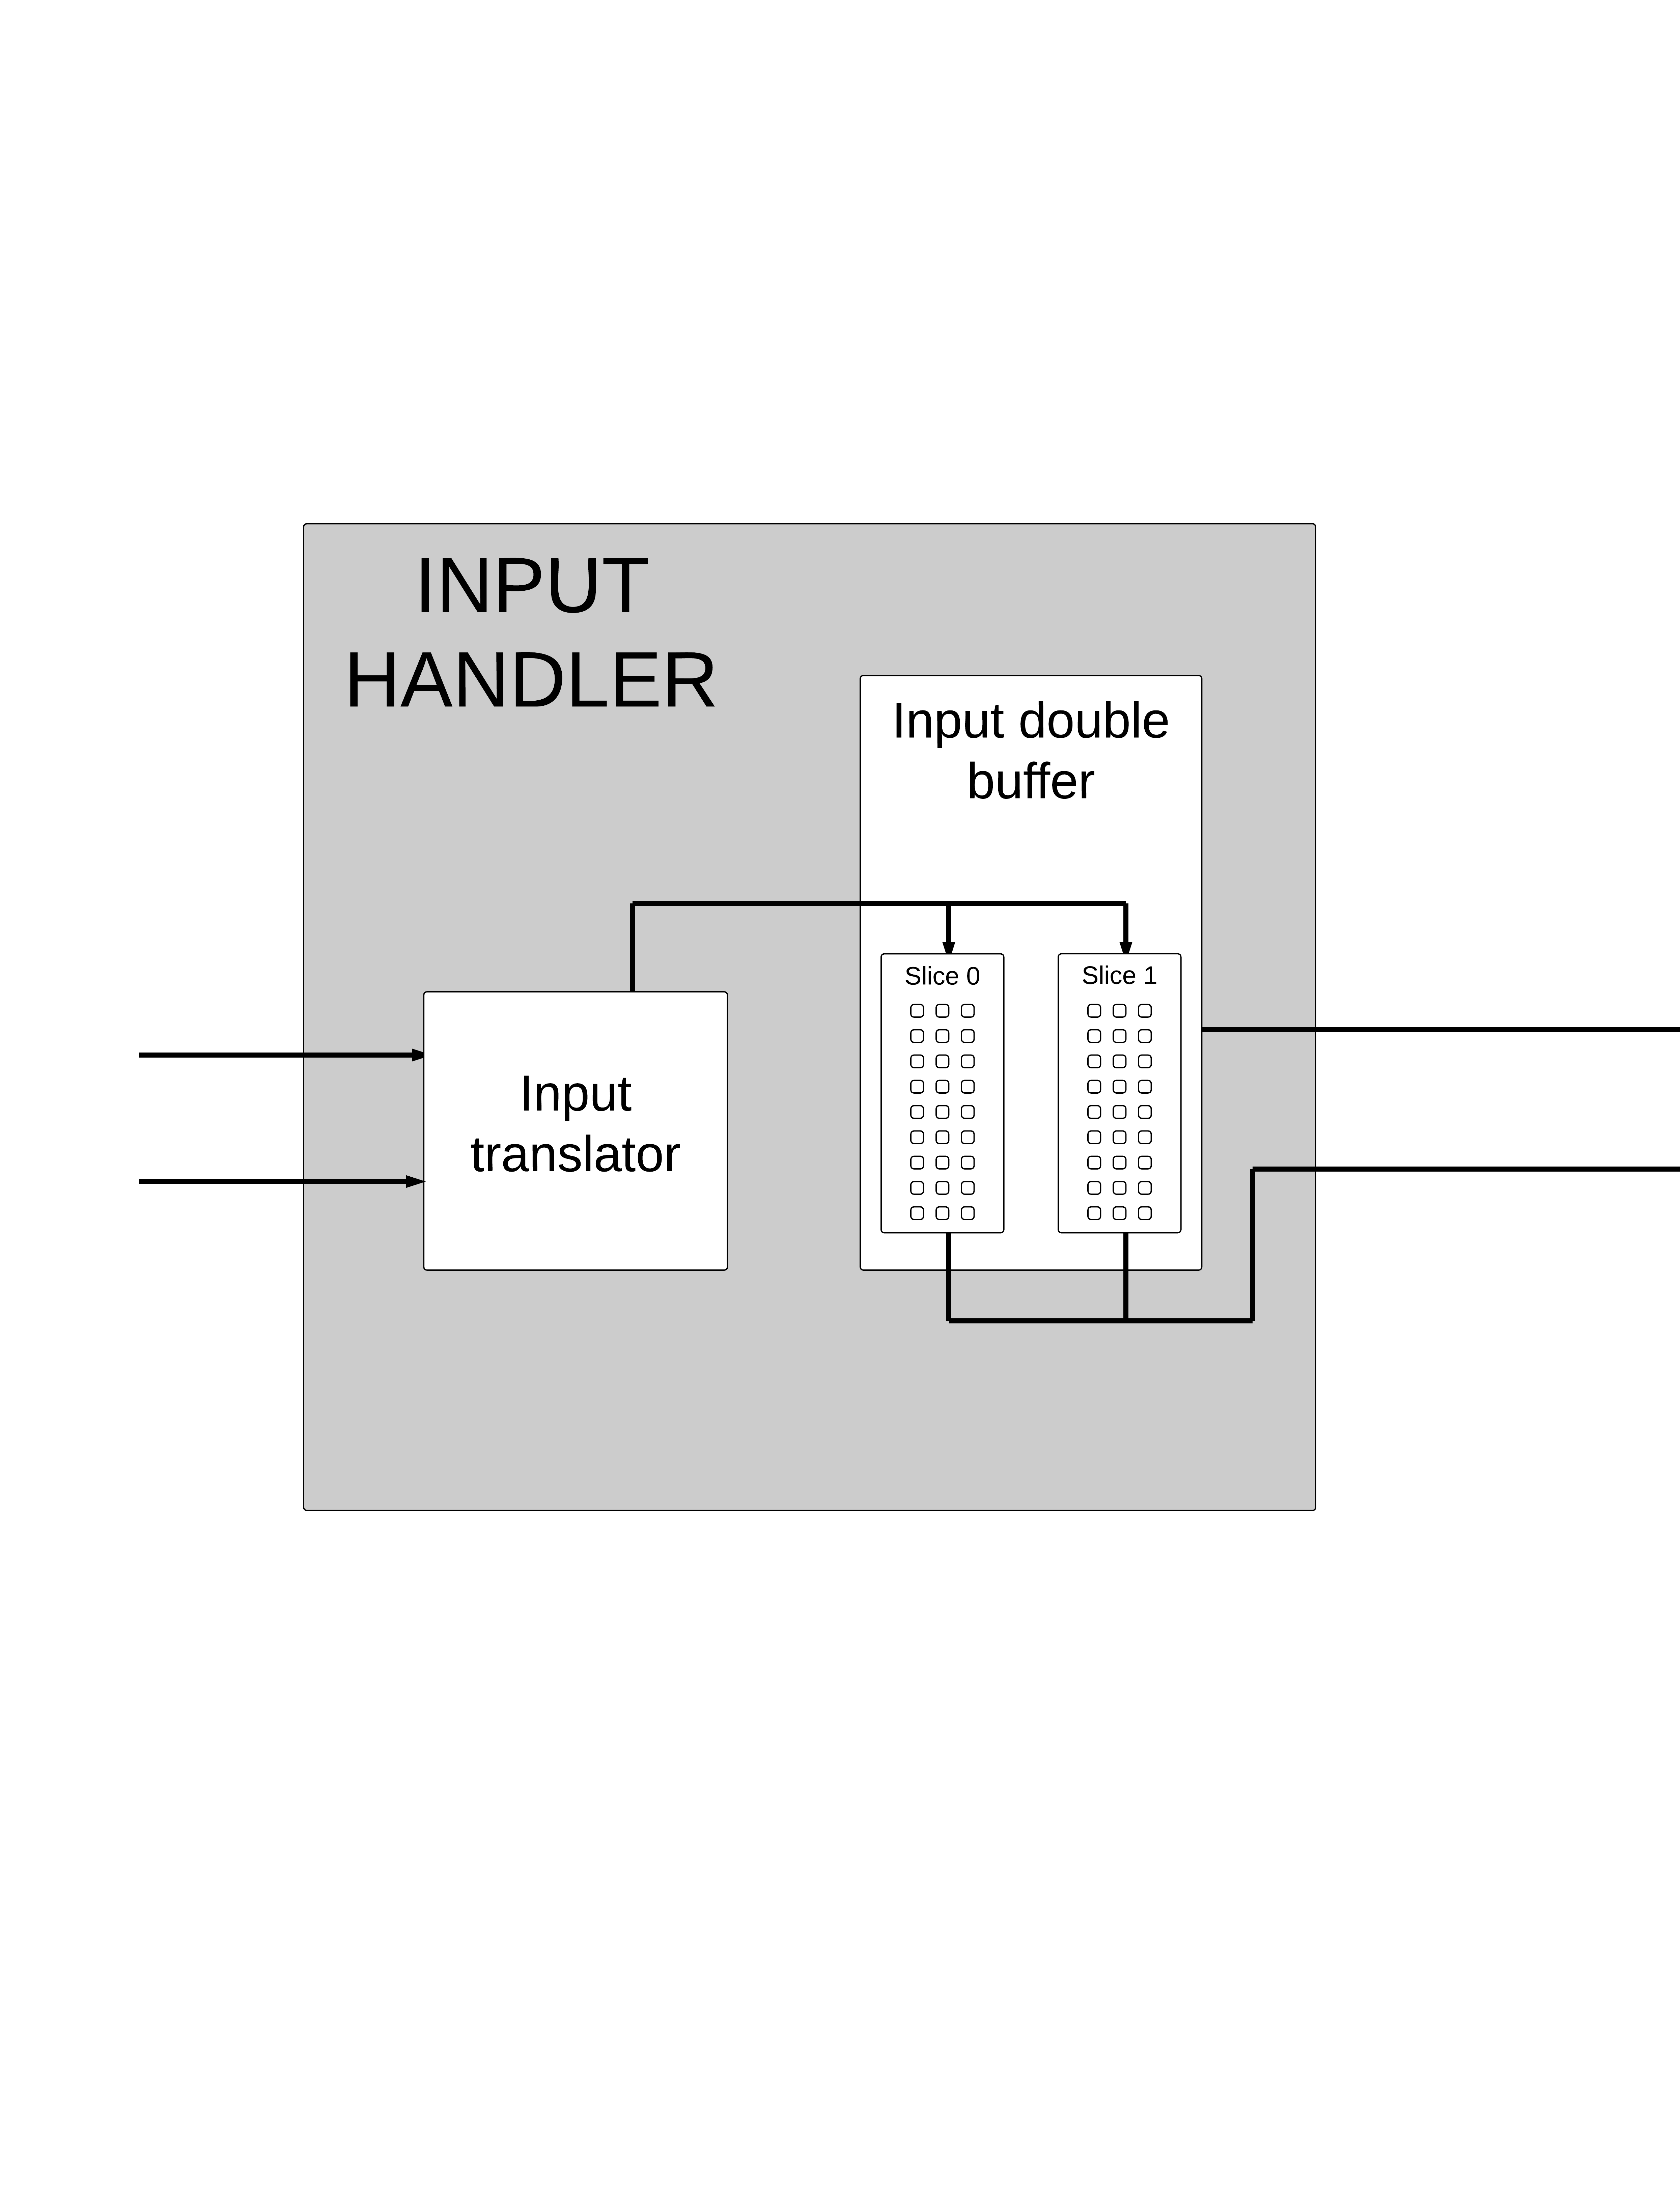
\includegraphics[width=\linewidth]{img/input_handler.png}
    \caption{Illustration of the input handler.}
    \label{fig:Convolution}
\end{figure}

        The processed input is then stored in a double buffer, allowing the input handler to both recieve data and feed the processor at the same time.
        As soon as a buffer is filled the input handler indicates that data is available to the processor and outputs data continously until the buffer is empty.
    \item[Processor] \hfill\\
        The processor recieves a pixel stream from the input handler and outputs convoluted data. It consists of a pixel buffer called the conveyor, a buffer for kernel data, an accumulator which performs the map and reduce operations, and a control module. In addition to providing convoluted data it also indicates that the data is valid.

\begin{figure}[h!]
    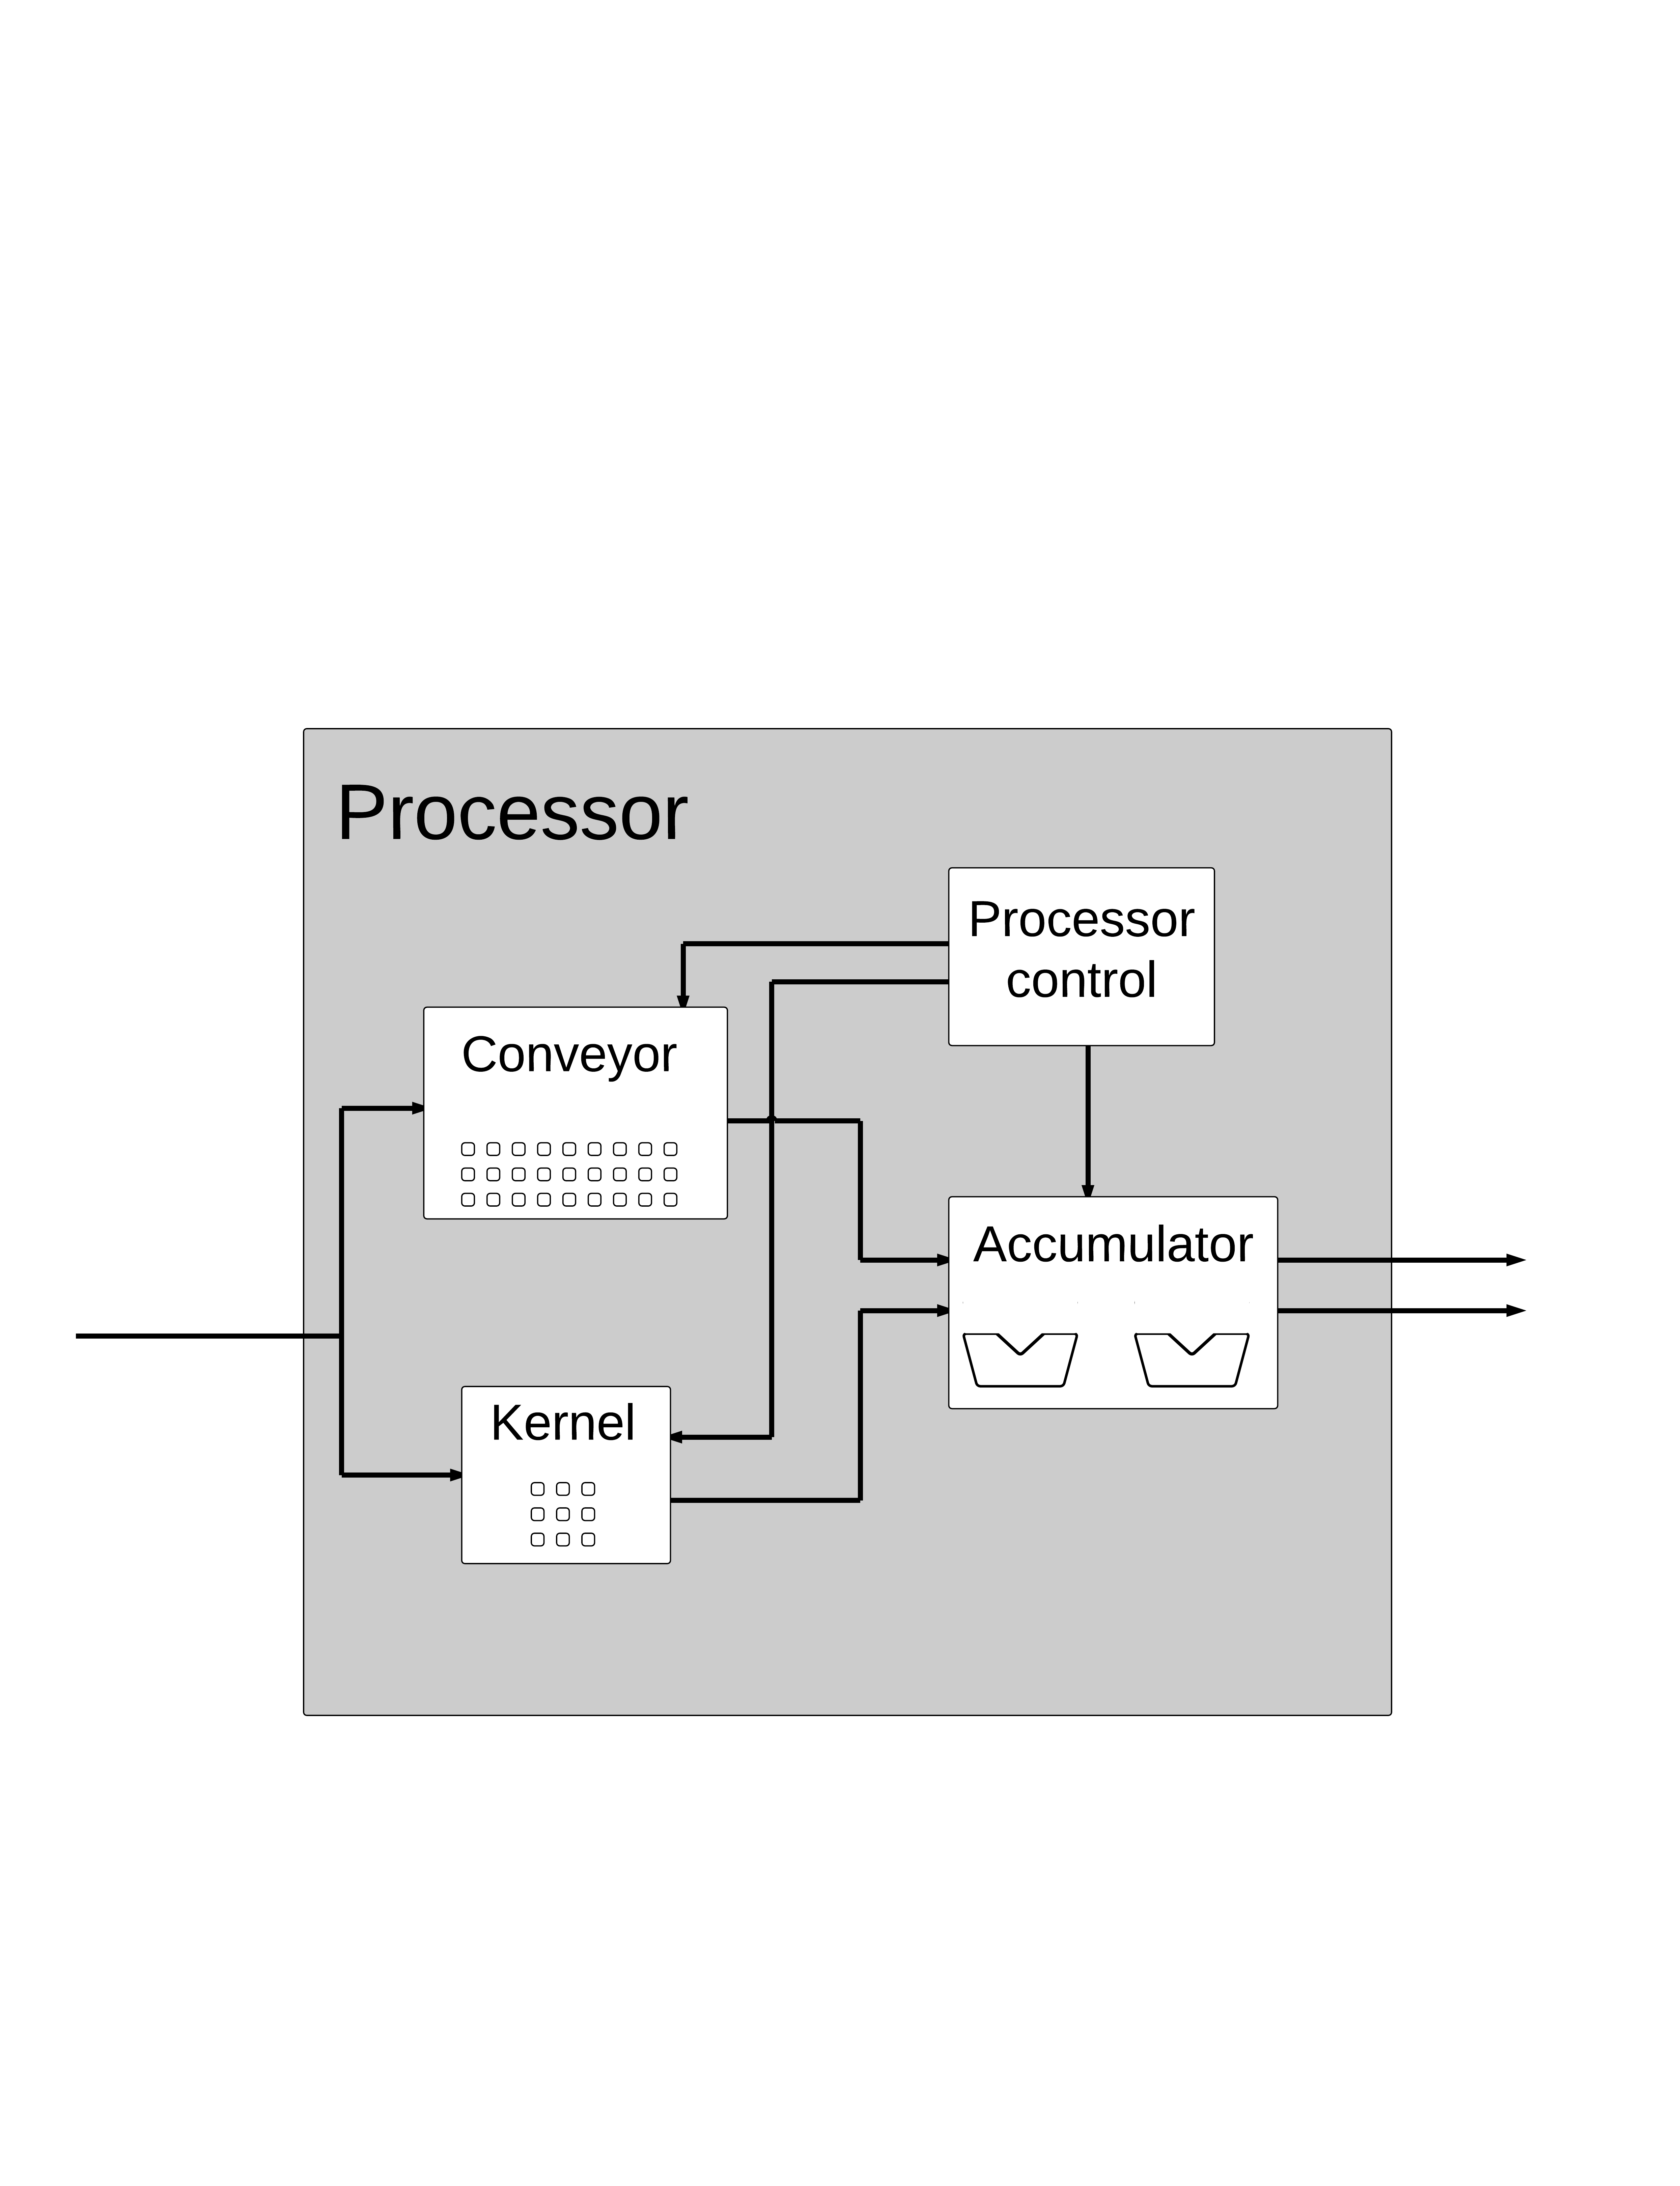
\includegraphics[width=\linewidth]{img/processor.png}
    \caption{Illusration of the processor.}
    \label{fig:Convolution}
\end{figure}

        This is nescessary because not all pixels entering the conveyor has access to their full neighbourhood, so the processor cannot provide valid output every cycle.
    \item[Control] \hfill\\
        The control module keeps track of the system state by monitoring the input data stream, and issues control signals according to the state.
        In its initial state the control module is in programming mode. 
        In this state the control module makes sure the initial instructions are dispatched to the correct modules before it enters data mode.
        When in data mode the controller keeps track of the data stream from the input handler, and uses this along with the valid signal from the processor to indicate to the output handler whether the output is valid or not.
    \item[Memory Control] \hfill\\
        Processed data is fed to one of the two SRAM chips serving as frame buffer. The output handler keeps track of which SRAM chip should be written to, and at which address.
\end{description}

TODO: This is where the overview should go. The next sections needs to be fleshed out A LOT!
The content below lacks context because this part is not yet done.

To illustrate how the components work we describe how the first frame of a videostream is processed.
\begin{enumerate}

    \item In its initial state the control module is in programming mode. It intercepts data from the input handler and fills the kernel buffer and decodes which map and reduction operation should be used
    \item After the instruction collected the control module enters data mode, and the input module starts filling its double buffer.
    \item When the input module has filled its first buffer it indicates that it is now outputting valid data which the processor will process.
    \item The control module keeps track of how much data has been fed to the processor. When the processor indicates it has valid output the control module signals the memory controller to be ready to write output to SRAM 0.
    \item When the input buffer is exhausted the control waits until all valid data has been flushed from the processor before it resets the processor and waits for the next buffer to fill.
    \item This cycle continues until the memory controller notices it has finished filling SRAM 0 with an entire frame. The memory controller switches to SRAM 1 and prepares for next frame.
\end{enumerate}

\subsection{Input handler}
\begin{figure}[h!]
    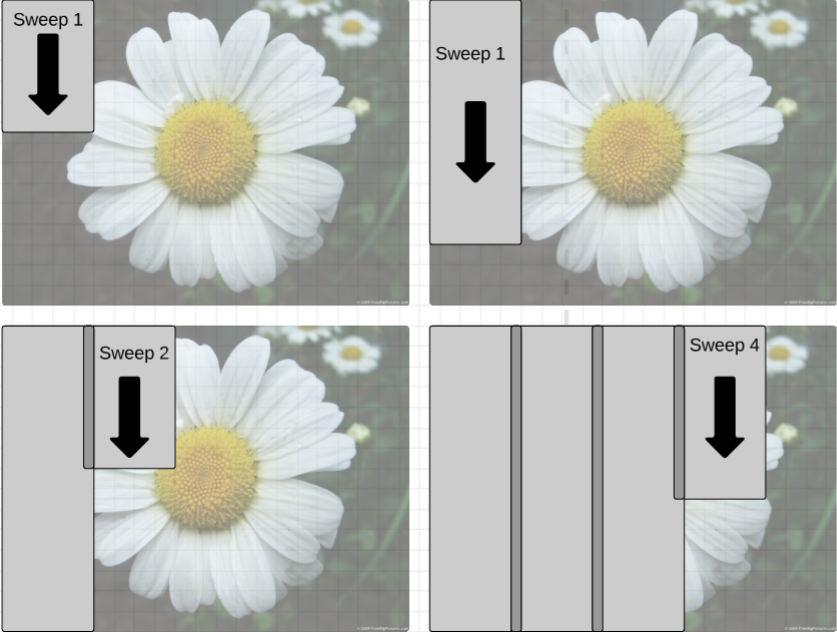
\includegraphics[width=\linewidth]{img/Sweeps.png}
    \caption{The sweep pattern used to collect data for convolution. The deep grey region indicates overlap, pixels which will be collected twice.}
    \label{fig:Sweeps}
\end{figure}
TODO describe how the input handlers work.

\begin{figure}[h!]
    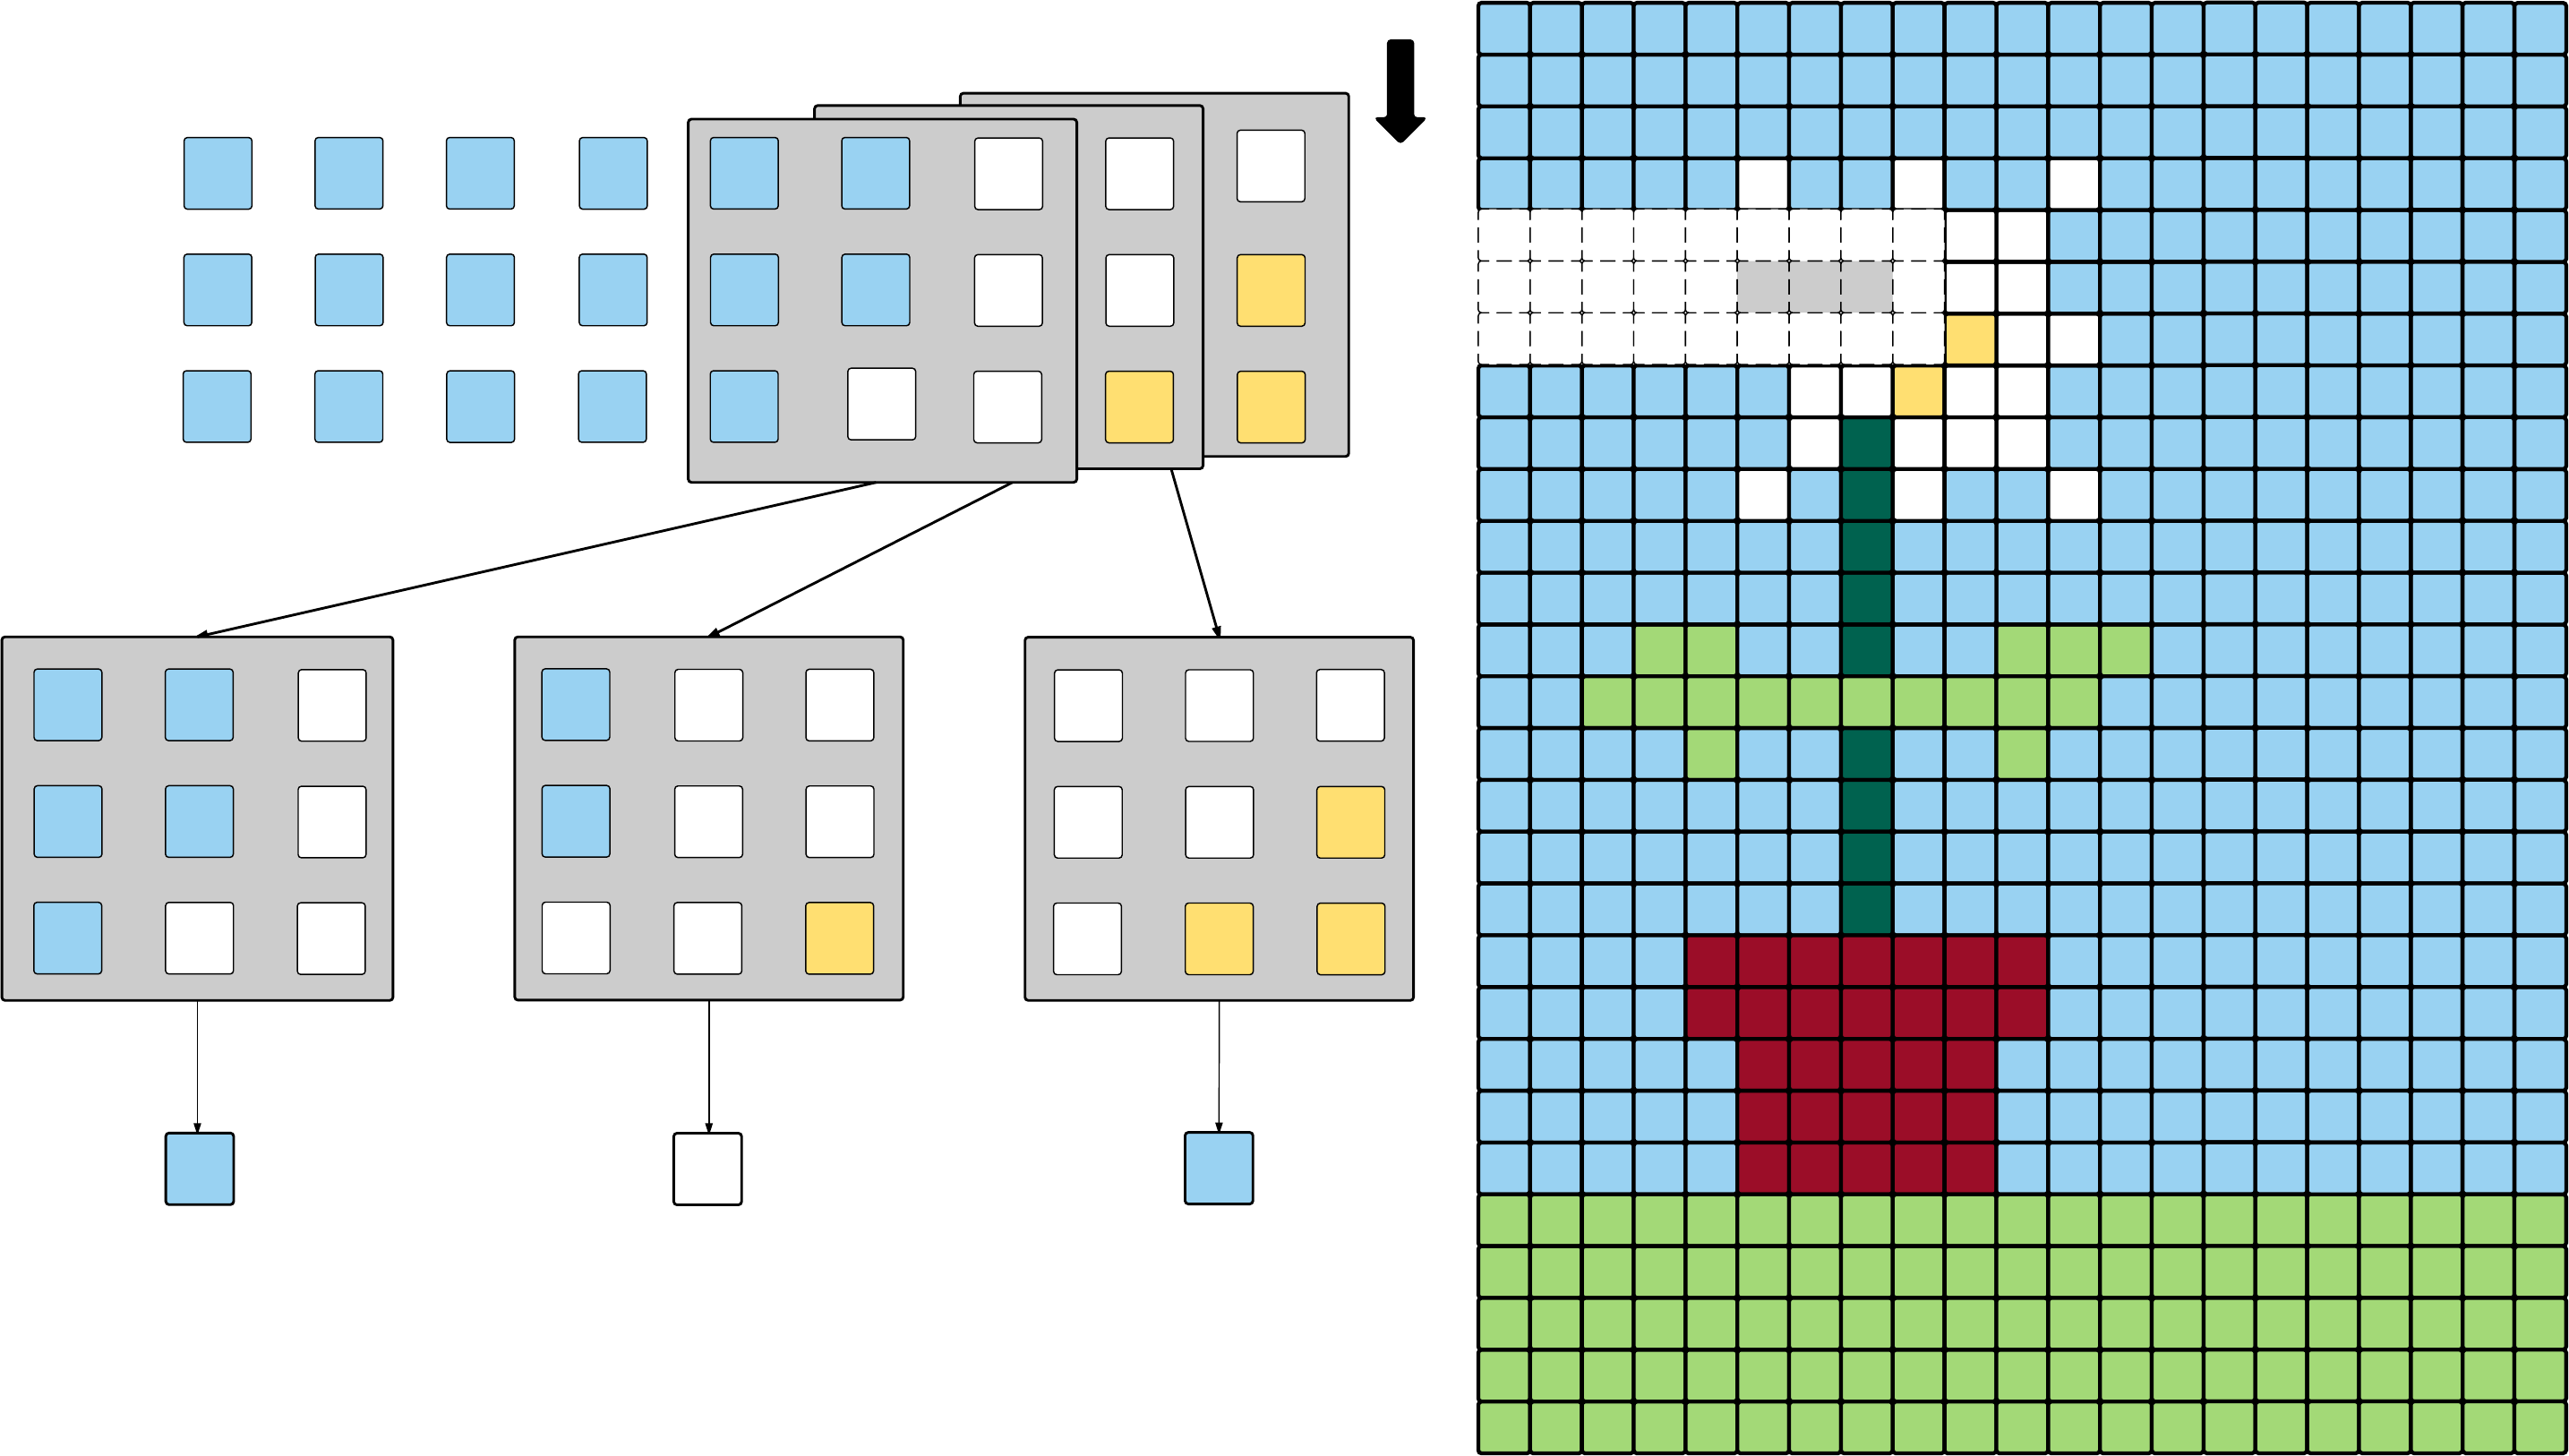
\includegraphics[width=\linewidth]{img/FeedPattern.png}
    \caption{The image three greyed out pixels in the source image represent the three pixels which the regions in grey boxes help calculate. The window is three pixels deep and nine pixels wide.}
    \label{fig:SweepFrontier}
\end{figure}

\subsection{Processor}

The processor recieves a data stream from the input handler and performs convolution on it, outputting a stream of convoluted image data.
The four main components are:
\begin{description}
    \item[Conveyor] \hfill\\ 
        The conveyor holds data in several rows, each one representing a column slice. The conveyor maintains these rows, moving data from row to row like a conveyor belt, and outputting data from each row to the accumulators.
    \item[The Kernel Buffer] \hfill\\
        The kernel buffer maintains the kernel data and must provide the correct kernel data for each map operation performed in the accumulators.
    \item[The Accumulator] \hfill\\
        The accumulator consists of several buffers, each buffer storing the progress of convoluting a pixel.
        Input to the accumulator is data from each row of the conveyor, along with kernel data from the kernel buffer, and it is up to the accumulator to make sure the correct kernel data and pixel data is mapped, and that the result is reduced with the content of the correct accumulator.
    \item[The Control Unit] \hfill\\
        In order for the accumulators and pixel conveyor to be in sync a control unit sends control signals periodically, which are then propogated throughout the system.
\end{description}

Figure \ref{fig:DaisyView} shows an overview of the four components in the heart of Daisy. 

\begin{figure}[h!]
    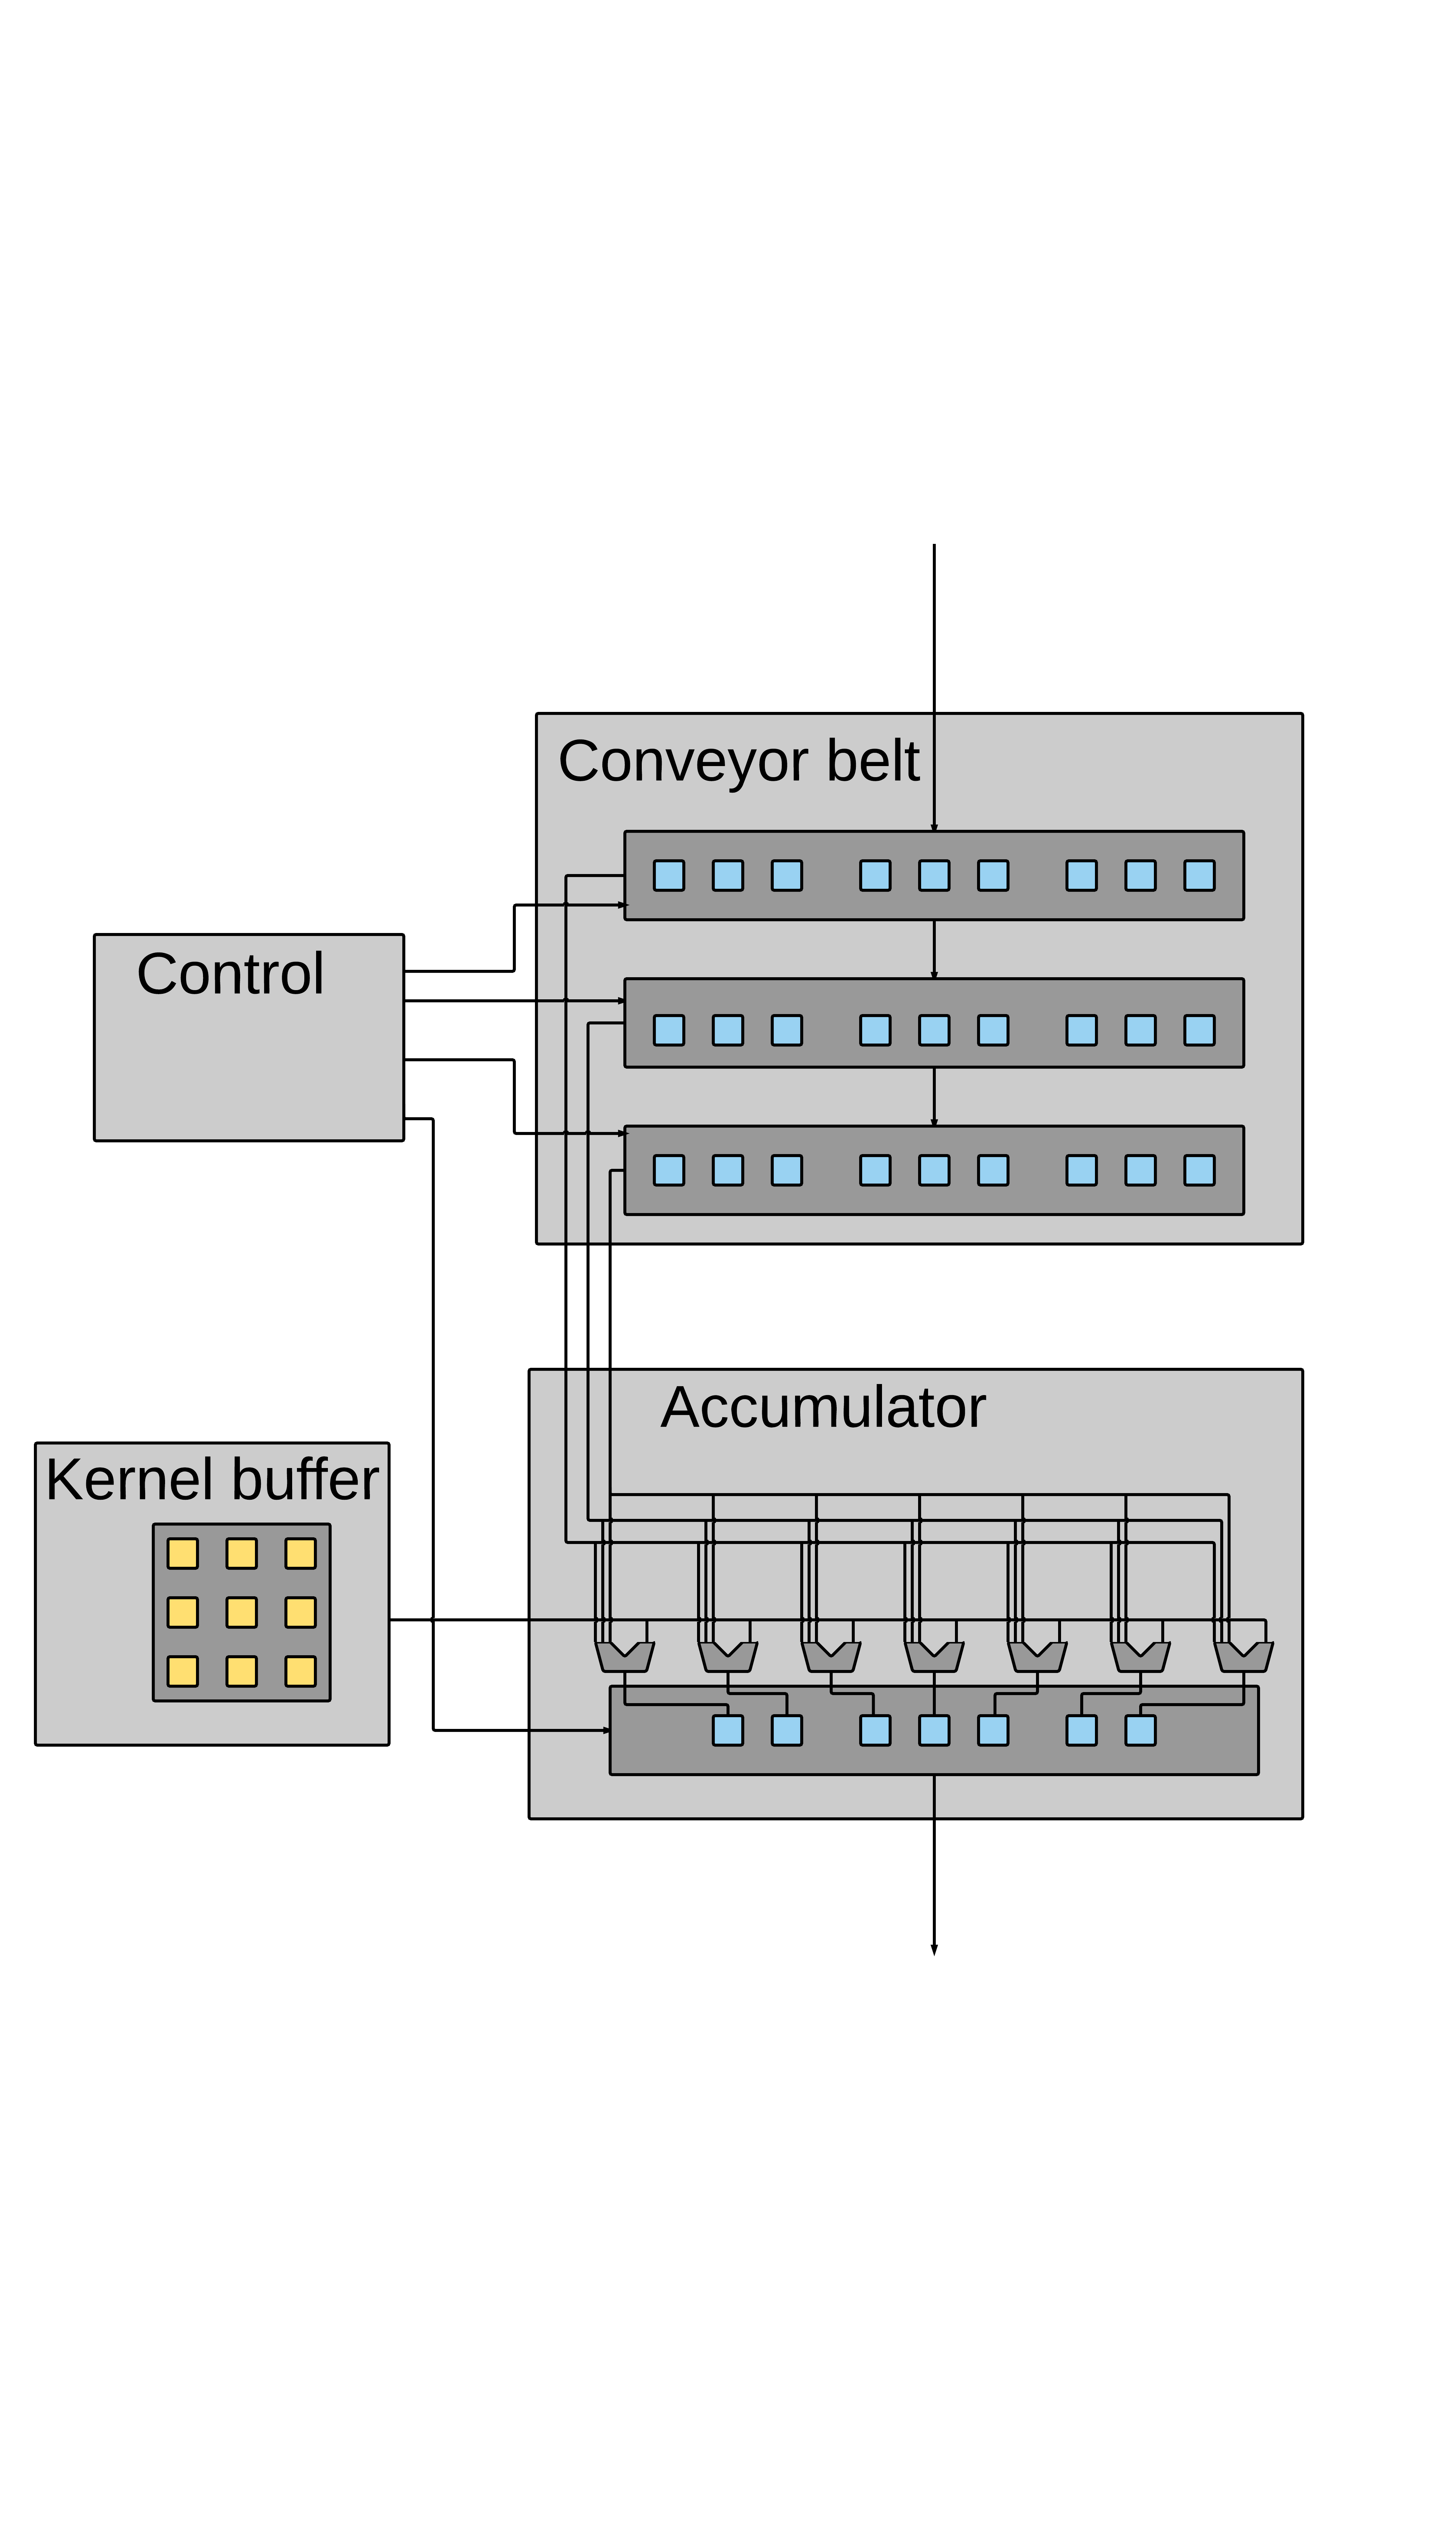
\includegraphics[width=\linewidth]{img/DaisyOverview.png}
    \caption{The four core units in the convolution process.}
    \label{fig:DaisyView}
\end{figure}

\subsubsection{The Accumulator}
Although the accumulator unit is the last unit in the datapath of Daisy we will cover it first since it helps motivate the designs further up in the chain.
The accumulator actually consists of seven accumulators, hereby referred to as pixel accumulators. Each pixel accumulator corresponds to a pixel in the middle row.
The leftmost and the rightmost pixel in the middle row has no accumulator associated with it because it lacks three pixels necessary for a full convolution, necessetating the slight overlap in our feed pattern.
In Figure \ref{fig:DaisyView} the input from the conveyor is shown as three wires, one from each row.  
Each accumulator is responsible to read from the correct row at the correct time, such that it accumulates only the subpixels of the source pixel.\\ \\ \\
\\
\begin{tabular}{l*{16}{c}r}
    Time (cycle)        & $T_{0}$ & $T_{1}$ & $T_{2}$ & $T_{2}$ & $T_{4}$  & $T_{5}$ & $T_{6}$ & $T_{7}$ & $T_{8}$ & $T_{9}$ & $T_{10}$ & $T_{11}$ & $T_{12}$ & $T_{13}$ & $T_{14}$\\
\hline
Row 1                   & 4 & 5 & 6 & 7 & 8 & 9 & \cellcolor{gray75} 1 & \cellcolor{gray75} 2 & \cellcolor{gray75} 3 & 4 & 5 & 6 & 7 & 8 & 9 & \\
Row 2                   & 7 & 8 & 9 & \cellcolor{gray75} 1 & \cellcolor{gray75} 2 & \cellcolor{gray75} 3 & 4 & 5 & 6 & 7 & 8 & 9 & \cellcolor{gray75} 1 & \cellcolor{gray75} 2 & \cellcolor{gray75} 3 & \\
Row 3                   & \cellcolor{gray75} 1 & \cellcolor{gray75} 2 & \cellcolor{gray75} 3 & 4 & 5 & 6 & 7 & 8 & 9 & \cellcolor{gray75} 1 & \cellcolor{gray75} 2 & \cellcolor{gray75} 3 & 4 & 5 & 6 & \\
\end{tabular}\\ \\ \\
We will first focus on the leftmost accumulator starting at time T0 doing the following reads. 
It first reads three values from Row 3 which corresponds to its southwestern subpixel at $T_{0}$, its southern subpixel at $T_{1}$, and its southeastern subpixel at $T_{2}$, shown as the greyed out cells in row 3.
At time $T_{3}$ it starts reading from Row 2, reading its western, middle and eastern subpixels at respectively $T_{3}$, $T_{4}$, and $T_{5}$, shown as the greyed out cells in row 2.
Finally it reads its northwestern, northern and northwestern subpixel at time $T_{6}$ to $T_{8}$ from Row 1.
What about the second leftmost accumulator then? By following the exact same read pattern, but waiting one cycle allows it to read all its values in the same manner as the leftmost accumulator!
The second accumulator reads from Row 3 at time $T_{1}$, switches to Row 2 at $T_{4}$ and again to Row 1 from $T_{7}$ to $T_{9}$. 
In fact, every accumulator starts one cycle later than its left neighbour, meaning every accumulator has accumulated its necessary pixels at different times.
\\ \\
\begin{tabular}{l*{16}{c}r}
    Time (cycle)        & $T_{0}$ & $T_{1}$ & $T_{2}$ & $T_{2}$ & $T_{4}$  & $T_{5}$ & $T_{6}$ & $T_{7}$ & $T_{8}$ & $T_{9}$ & $T_{10}$ & $T_{11}$ & $T_{12}$ & $T_{13}$ & $T_{14}$\\
\hline
Row 1                   & \cellcolor{gray75} 4 & 5 & 6 & 7 & 8 & 9 & 1 & \cellcolor{gray75} 2 & \cellcolor{gray75} 3 & 4\cellcolor{gray75} & 5 & 6 & 7 & 8 & 9 & \\
Row 2                   & 7 & 8 & 9 & 1 & \cellcolor{gray75} 2 & \cellcolor{gray75} 3 & \cellcolor{gray75}4 & 5 & 6 & 7 & 8 & 9 & 1 & \cellcolor{gray75} 2 & \cellcolor{gray75} 3 & \\
Row 3                   & 1 & \cellcolor{gray75} 2 & \cellcolor{gray75} 3 & 4\cellcolor{gray75} & 5 & 6 & 7 & 8 & 9 & 1 & \cellcolor{gray75} 2 & \cellcolor{gray75} 3 & 4\cellcolor{gray75} & 5 & 6 & \\
\end{tabular}\\ \\ \\

\subsubsection{The Conveyor Belt}
As established last section, the job of the conveyor is to feed data from each of its rows to the accumulator.
In addition to serving data to the accumulator the conveyor must also feed new data to the belt and propogate that data downward which gives rise to its name.
In order to both propagate data downward and feed correct data to the accumulator as efficently as possible the conveyor will utilize the data from a read operation to both feed the accumulator and to transfer data laterally.
When a register is read, it is therefore the job of the register directly beneath it to read, conveying data downwards.
By studying the tables in the previous section we see that reads are done in a wave pattern, and consequentially so is the data conveying, which has a very powerful implication:
Since every accumulator and register will perform the same operation as its left neighbour offset by one cycle we can let each element be responsible for controlling the element to its right.
Rather than using a central control module we can instead simply daisy chain the control signals and interface only with the leftmost components, which also explains the name of the convolution core, Daisy.
An analogy to the read signals is a key. At time $T_{0}$ the control element gives the leftmost register the read key. 
The register does as it is told and reads its new value from the register above, and hands the key over to its neighbour. 
At $T_{1}$ the neighbour recieves the key, and reads from the register above it and sends the key further on.

TODO: Figure out a succint way to explain this part

\subsubsection{The Controller}
We have established how control flows throughout the system, but we still need a module to give out keys to the leftmost accumulators and registers.
The controller is responsible for sending out the keys in the correct order and at the correct time.
Timing is everything, if we misalign read signals and write signals we may end up in a situation where a register fails to read when the register above it writes.
For example, if the controller sends each read signal one cycle too late each register will read when the register to the right side of the one directly above it, causing the data to be sheared as it moves laterally!
Other than issuing read and write keys to the registers, the controller also issues a flush key for the accumulators which tells accumulators to drive DATA\_OUT with its contents, and to reset.

\subsubsection{The Kernel Buffer}
In our schematic we present the kernel buffer as a separate submodule. 
However, having already introduced how instructions are daisy chained it makes sense to do the same with kernels since seven different kernel values are in use at all times.
Thus the kernel values are kept in a shift register queue living as close to the accumulators as possible, needing only two registers to hold the currently unused kernel values.
The responsibilities of the kernel unit is thus to collect the first data values into the kernel buffer chain and to buffer the two kernel values which are not currently in use.
